\section{ハード構成}\label{dux30d7ux30eaux30f3ux30bfux306eux57faux672cux539fux7406}

本章では、かわさきロボット大会指定の380モータではなく、
手っ取り早くモータ制御を実現するために、市販されているハード(Fig.\ref{fig201})で構成しました。
全てのハードは通販サイト、例えばスイッチサイエンス \cite{switch-science_HP} から購入できます。
既存のハードでモータ制御を学んだのちに、ロボット本体へ適用します。

\begin{itemize}
    \tightlist
    \item
    マイコン:Arduino Mega 2560 R3
    \item
    モータドライバ:VNH5019搭載モータードライバ (POLOLU-1451)
    \item
    モータ:75:1 シャフト付き超小型メタルギアドモーター HP (POLOLU-2215)
    \end{itemize}

\begin{figure}[htbp]
\centering
\includegraphics[width=300pt]{fig/fig201.eps}
\caption{ハード構成}
\label{fig201}
\end{figure}


\section{回路図}\label{ux71b1ux6eb6ux89e3ux7a4dux5c64ux6cd5fdm}

回路図は、Fig.\ref{fig202}の通りです。
Arduino Mega 2560 のピン5~7を使用してモータドライバを動かします。
モータドライバ VNH5019 の詳細は、
Pololu HP \cite{pololu_HP_driver} に記載されています。

\begin{figure}[htbp]
\centering
\includegraphics[width=350pt]{fig/fig202.eps}
\caption{回路図}
\label{fig202}
\end{figure}


\section{Simulinkモデル}\label{ux71b1ux6eb6ux89e3ux7a4dux5c64ux65b9ux6cd5ux306eux7279ux5fb4}

Simulinkモデルは、Fig.\ref{fig203}の通りです。
ArduinoをSimulink上で実行できるように、シミュレーションモードを "エクスターナル" に、
シミュレーション終了時間を "inf" に変更します。

コンフィギュレーション パラメーターを開き、
ハードウェア実行 ⇒ ハードウェア ボードを "Arduino Mega 2560" にします(Fig.\ref{fig204})。

指令値をモータドライバの制御信号に変換するために、MATLAB Function ブロックを使用します。
ブロックの中身は、Fig.\ref{fig205}の通りです。
プロポからのラジコン信号入力を想定して、1500usec付近でモータ停止、
1150~1850usecの間で速度変更する仕様としてます。

\begin{figure}[htbp]
\centering
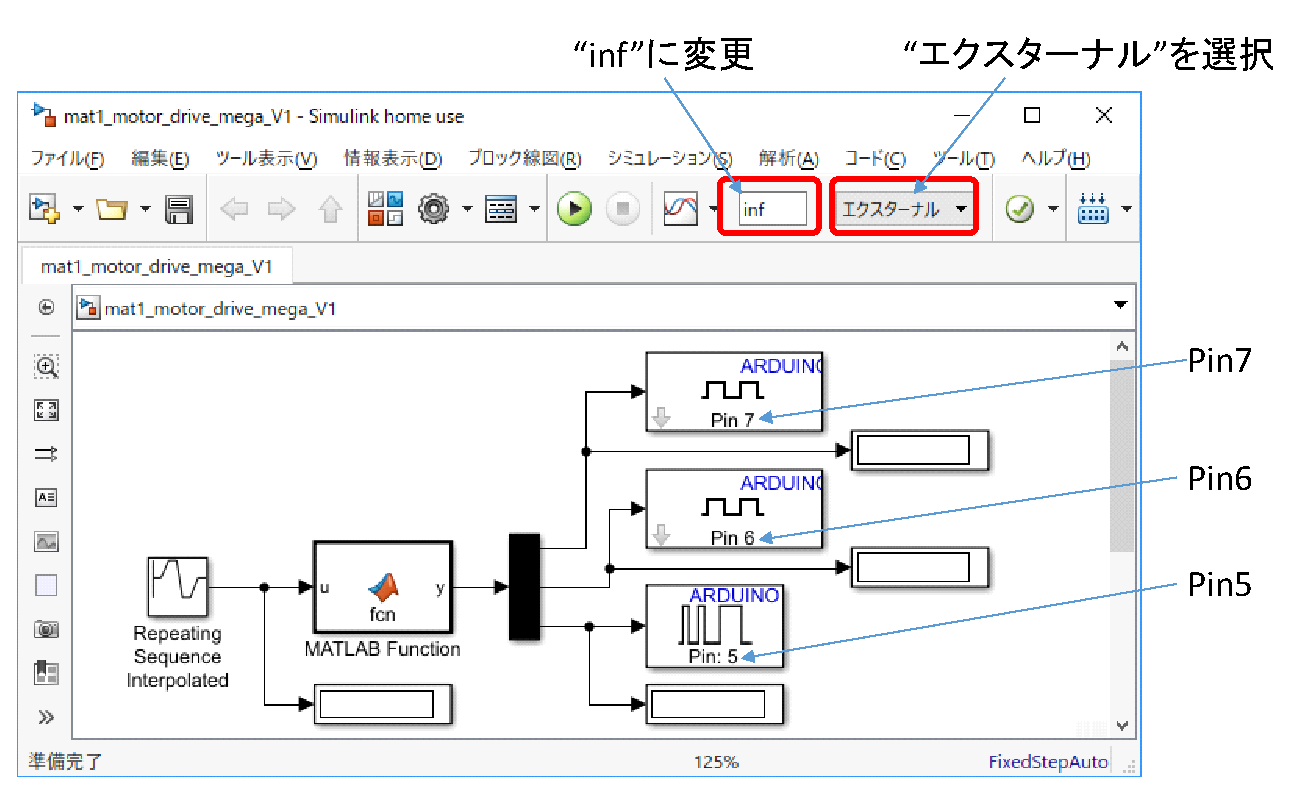
\includegraphics[width=350pt]{fig/fig203.eps}
\caption{Simulinkモデル}
\label{fig203}
\end{figure}

\begin{figure}[htbp]
\centering
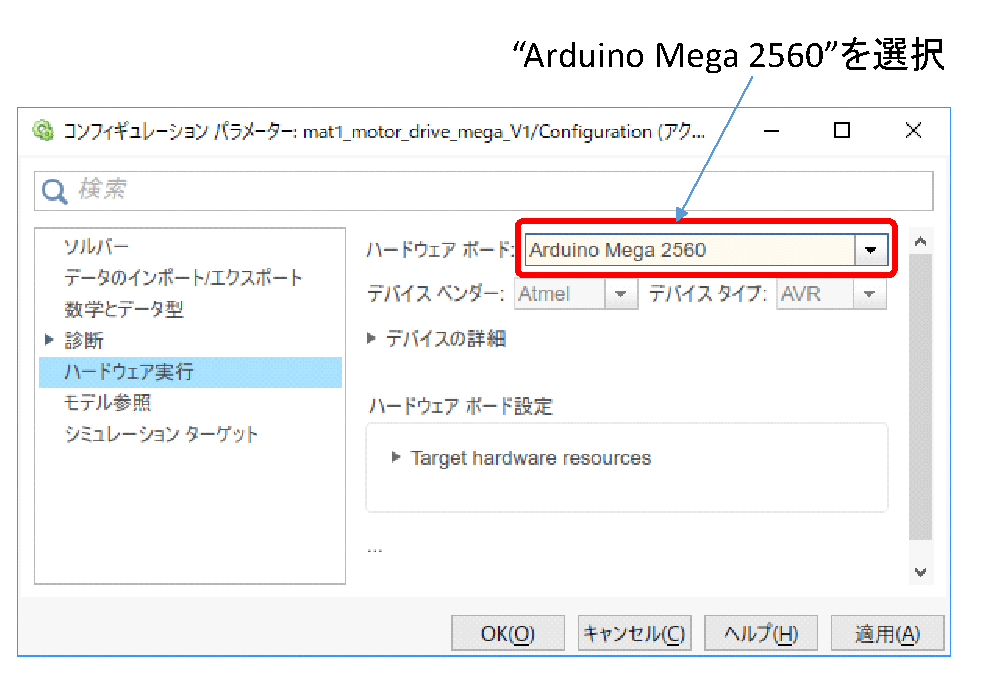
\includegraphics[width=300pt]{fig/fig204.eps}
\caption{コンフィギュレーション パラメーター}
\label{fig204}
\end{figure}

\begin{figure}[htbp]
\centering
\includegraphics[width=380pt]{fig/fig205.eps}
\caption{MATLAB Function ブロックの中身}
\label{fig205}
\end{figure}


\clearpage
\section{実行}\label{dux30d7ux30eaux30f3ux30bfux306eux57faux672cux7684ux306aux69cbux9020}

Fig.\ref{fig206}に示すボタンをクリックすることでプログラムを実行できます。

Simulinkと連動して動作させる場合は "実行" をクリックします。
ビルドに成功して動作し始めると、Display ブロックに出力値がリアルタイムに表示されます。
また、入力値として使用した Repeating Sequence Interpolated ブロックをダブルクリックし、
パラメータを変更することで、実行しながらもパラメータ変更の挙動が確認できます。

Simulinkと連動させず、Arduinoをスタンドアロンで動かす場合は "ハードウェアに展開" をクリックします。
一度書き込めば、Simulinkと接続しなくてもプログラムが動くようになります。

\begin{figure}[htbp]
\centering
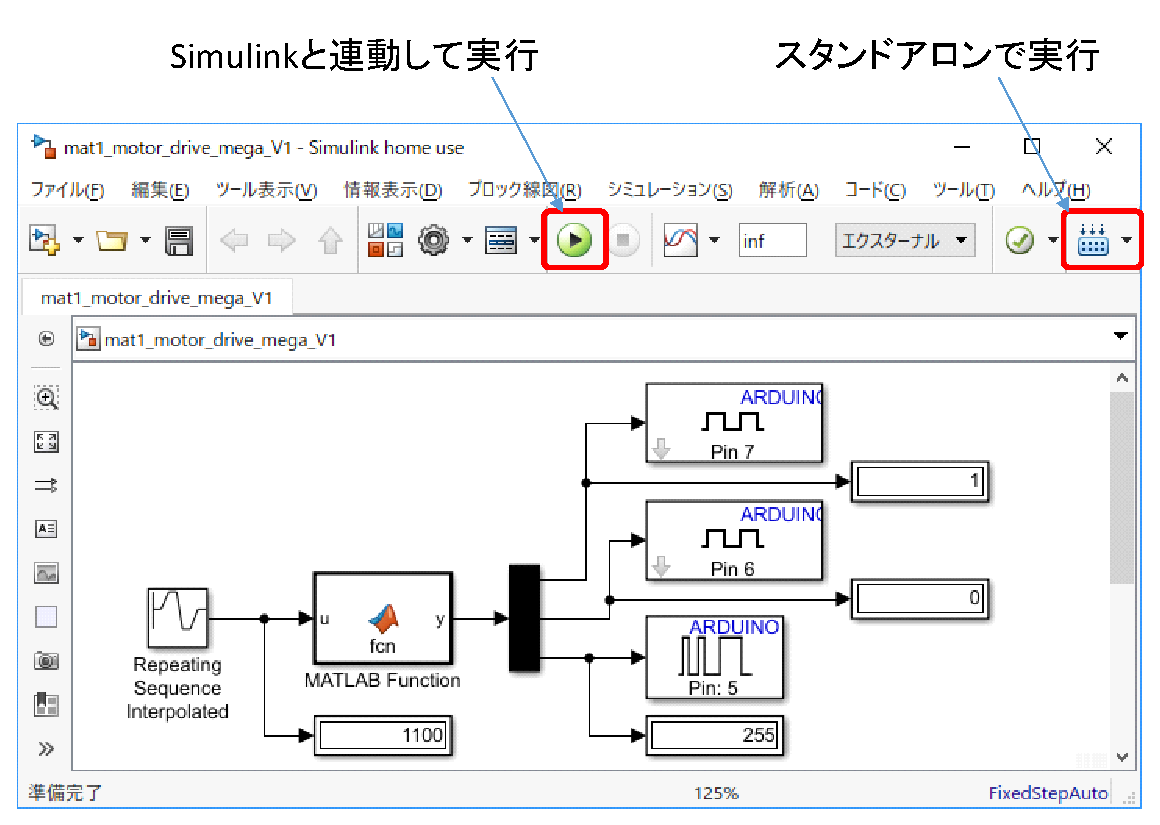
\includegraphics[width=350pt]{fig/fig206.eps}
\caption{Matlab/Simulinkモデルの実行}
\label{fig206}
\end{figure}
